\chapter{Arhitektura i dizajn sustava}

	Arhitektura aplikacije može se podijeliti na četiri podsustava:
	\begin{itemize}
		\item Web poslužitelj
		\item Web aplikacija
		\item Baza podataka
		\item Mobilna aplikacija
	\end{itemize}

	\begin{figure}[H]
		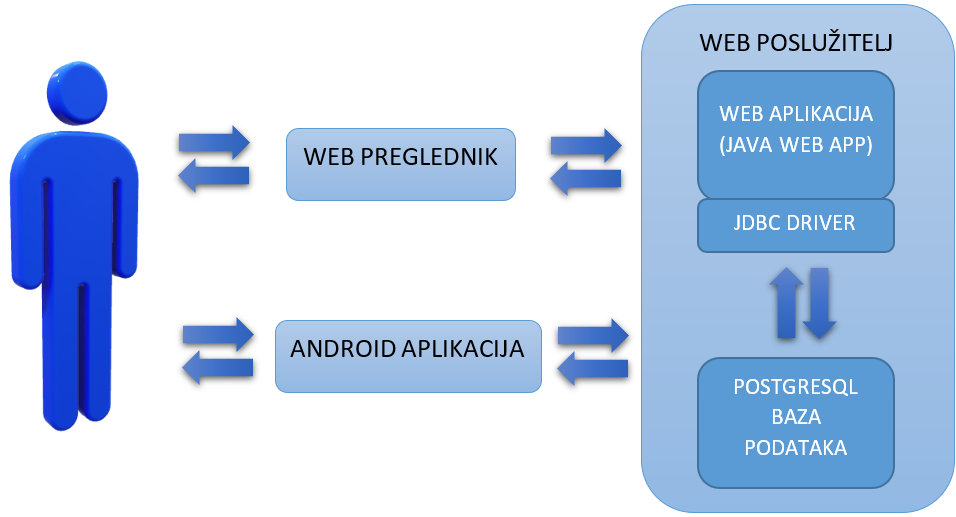
\includegraphics[scale=0.7]{Slike/Arhitektura sustava.PNG}
		\centering
		\caption{Arhitektura sustava s prikazom podsustava i toka podataka}
		\label{fig:dijagramSustava}
	\end{figure}

	\textit{\underline{Web poslužitelj}} osnova je web aplikacije. To je računalo koje preko internetske mreže uspostavlja komunikaciju s korisnicima sustava. U našem slučaju, to je Windows Server virtualna mašina podignuta preko servisa Microsoft Azure. Na njemu su instalirani svi servisi koji su potpora radu web aplikacije i baze podataka.
	
	\textit{\underline{Web aplikacija}} mozak je našeg sustava. U njoj je opisana sva logika aplikacije. Razgovara sa korisnikom sustava putem HTTP (engl. \textit{Hyper
	Text Transfer Protocol}) protokola, obrađuje zahtjeve, spaja se s bazom podataka te šalje odgovor korisniku na web preglednik ili Android aplikaciju. Odgovor je oblika HTML dokumenta u slučaju korištenja web preglednika ili oblika JSON (JavaScript Object Notation) dokumenta u slučaju spajanja Android aplikacije na RESTful API sustava.

	Za backend sustava odabran je programski jezik Java te tehnologije Java Servleti i JSP (Java Server Pages). Backend je pisan kao Maven projekt radi lakšeg upravljanja ovisnostima naše aplikacije. Kao razvojno okruženje koristi se IDE Eclipse, a Apache Tomcat kao Servlet container.
	
	Oblikovnim obrascem MVC (Model-View-Controller) ostvarili smo razdvajanje frontend i backend dijela sustava te njihovo nezavisno i paralelno razvijanje. Posljedica toga jest jednostavno testiranje i utvrđivanje grešaka sustava te jednostavna buduća nadogradnja.
	
	Obrazac MVC sastoji se od tri komponente:
	\begin{packed_item}
		
		\item \textbf{Model} - strukture podataka koje služe preslikavanju podataka iz baze u objektno orijentiran jezik. Omogućuju lakši dohvat i lakše upravljanje podacima spremljenim u bazu.
		\item \textbf{View} - komponenta koja služi prikazu podataka iz modela na korisniku razumljiv i jednostavan način. U slučaju naše web aplikacije, za to je zadužena tehnologija JSP.
		\item \textbf{Controller}
		
	\end{packed_item}
	
	Odabrali smo relacijski model \textit{\underline{baze podataka}} zbog njegove raširenosti, jednostavnosti i skalabilnosti. Bazu podataka opisali smo jezikom SQL i pokrenuli ju na sustavu PostgreSQL.

	\textit{\underline{Mobilna aplikacija}} još jedan je pogled korisnika u naš sustav. Ona je izgrađena u programskom jeziku Java koristeći Android studio kao IDE. Mobilna aplikacija spaja se na RESTful dio web poslužitelja preko kojeg vrši prijavu u sustav i dohvaćanje podataka. Za izradu dizajna Android aplikacije koristi se sustav Adobe XD i Google Material Design kao vizualni jezik.
		
		\eject
				
		\section{Baza podataka}
			
			
		Za potrebe našeg sustava koristit ćemo SQL relacijsku bazu podataka. Relacijska baza podataka najviše nam odgovara zbog olakšanog modeliranja događaja i entiteta iz stvarnog svijeta. Osnovna jedinka baze podataka je relacija, to jest tablica koja ima svoj naziv i potreban skup atributa. Zadaća baze podataka je brza i jednostavna pohrana, izmjena i dohvat podataka koje potom treba obraditi. Sve su relacije u bazi svedene na treću normalnu formu kako baza ne bi sadržavala redundantne podatke. Prilikom izrade baze podataka poslužili smo se PostgreSQL-om.
		Baza podataka ove aplikacije sastoji se od sljedećih entiteta:
		\begin{itemize}
			\item 	Profil
			\item 	Korisnički račun
			\item 	Registracija klijenta
			\item   Razina ovlasti
			\item   Kredit
			\item   Vrsta kredita
			\item   Transakcija
			\item   Račun
			\item   Vrsta računa
			\item   Kartica
			\item   Vrsta kartice	
			\item   Mjesto
			\item   Županija	
		\end{itemize}
		
		\eject
		
			\subsection{Opis tablica}
			

				\textbf{Profil} Ovaj entitet sadrži sve važne informacije za pristup web aplikaciji. Sadrži atribute: ime, prezime, OIB, adresa prebivališta, poštanski broj, datum rođenja, e-mail adresa i slika profila. Ovaj entitet u vezi je \textit{Zero-to-Many} s entitetom Korisnički račun preko OIB-a i u vezi je \textit{Many-to-One} sa entitetom Mjesto preko poštanskog broja. Također je i u vezi sa \textit{One-to-One} sa entitetom Registracija klijenta preko OIB-a.
				
				\begin{longtabu} to \textwidth {|X[8, l]|X[8, l]|X[16, l]|}
					
					\hline \multicolumn{3}{|c|}{\textbf{Profil }}	 \\[3pt] \hline
					\endfirsthead
					
					\hline \multicolumn{3}{|c|}{\textbf{Profil}}	 \\[3pt] \hline
					\endhead
					
					\hline 
					\endlastfoot
					
					Ime & VARCHAR	&  	ime korisnika\cellcolor{LightGreen} 	\\ \hline
					Prezime	& VARCHAR &  prezime korisnika 	\\ \hline 
					\rowcolor{lightgreen}\textbf{OIB} & VARCHAR &  OIB korisnika \\ \hline 
					Adresa prebivališta & VARCHAR &   adresa korisnika      \\ \hline
					\textit{Poštanski broj} & INT & poštanski broj (mjesto.poštanskiBroj) \\ \hline
					Datum rođenja & DATE & datum rođenja korisnika \\ \hline
					Email & VARCHAR & e-mail adresa korisnika \\ \hline
					Slika & VARCHAR & slika korisnika \\ \hline
					
					 
					
					
				\end{longtabu}
			
			\textbf{Korisnički Račun}  Ovaj entitet sadrži sve važne informacije o korisničkom računu. Sadrži atribute: OIB, korisničko ime, lozinka, razina ovlasti i promjena lozinke. Ovaj entitet je u vezi \textit{Many-to-Zero} s entitetom Profil preko OIB-a i s entitetom \textit{{One-to-One}} Razina ovlasti preko razine ovlasti. 
			
			\begin{longtabu} to \textwidth {|X[8, l]|X[8, l]|X[16, l]|}
				
				\hline \multicolumn{3}{|c|}{\textbf{Korisnički račun }}	 \\[3pt] \hline
				\endfirsthead
				
				\hline \multicolumn{3}{|c|}{\textbf{Korisnički račun}}	 \\[3pt] \hline
				\endhead
				
				\hline 
				\endlastfoot
				
				\cellcolor{LightGreen}\textbf{Korisničko ime} & VARCHAR	&  jedinstveni identifikator korisnika \\ \hline
				Lozinka	& VARCHAR &   hash lozinke	\\ \hline 
				\textit{OIB} & VARCHAR & OIB korisnika (profil.OIB)\\ \hline
				\textit{Razina ovlasti} & INT & broj razine ovlasti (razinaOvlasti.razinaOvlasti)\\ \hline
				Promjena lozinske & BOOLEAN & treba li promijeniti lozinku prilikom prijave \\ \hline
				
			\end{longtabu}
		

		\eject
		
				\textbf{Registracija klijenta}  Ovaj entitet sadrži sve važne informacije o registraciji klijenta. Sadrži atribute: OIB i privremeni ključ. Ovaj entitet je u vezi \textit{One-to-One} s entitetom Profil preko OIB-a.
			
			\begin{longtabu} to \textwidth {|X[8, l]|X[8, l]|X[16, l]|}
				
				\hline \multicolumn{3}{|c|}{\textbf{Registracija klijenta }}	 \\[3pt] \hline
				\endfirsthead
				
				\hline \multicolumn{3}{|c|}{\textbf{Registracija klijenta}}	 \\[3pt] \hline
				\endhead
				
				\hline 
				\endlastfoot
				
				\textit{OIB} & VARCHAR & OIB korisnika (profil.OIB)\\ \hline
				Privremeni ključ & VARCHAR & privremeni ključ prilikom otvaranja računa \\ \hline
				
			\end{longtabu}
			
			
			
		
		
			
		\textbf{Razina ovlasti}  Ovaj entitet sadrži informacije vezane za razinu ovlasti. Sadrži atribute: razina ovlasti i naziv. Ovaj je entitet u vezi \textit{One-to-One} s entitetom Korisnički račun preko razine ovlasti.  
		
		\begin{longtabu} to \textwidth {|X[8, l]|X[8, l]|X[16, l]|}
			
			\hline \multicolumn{3}{|c|}{\textbf{Razina ovlasti}}	 \\[3pt] \hline
			\endfirsthead
			
			\hline \multicolumn{3}{|c|}{\textbf{Razina ovlasti}}	 \\[3pt] \hline
			\endhead
			
			\hline 
			\endlastfoot
			
		    \textbf{Razina ovlasti} & INT & Broj razine ovlasti  \\ \hline
			Naziv & VARCHAR	& Naziv ovlasti	\\ \hline
			
			
			
			
			
		\end{longtabu}
	
		\textbf{Mjesto} Ovaj entitet sadrži sve važne informacije o mjestu. Sadrži atribute: poštanski broj, naziv mjesta i šifra županije. U vezi je \textit{One-to-Many} s entitetom Profil preko poštanskog broja i u vezi \textit{Many-to-One} s entitetom Županija preko šifre županije.
			\begin{longtabu} to \textwidth {|X[8, l]|X[8, l]|X[16, l]|}
		
		\hline \multicolumn{3}{|c|}{\textbf{Mjesto}}	 \\[3pt] \hline
		\endfirsthead
		
		\hline \multicolumn{3}{|c|}{\textbf{Mjesto}}	 \\[3pt] \hline
		\endhead
		
		\hline 
		\endlastfoot
		
		\textbf{Poštanski broj} & INT & poštanski broj mjesta \\ \hline
		Naziv mjesta & VARCHAR & naziv mjesta \\ \hline
		\textit{Šifra županije} & INT & šifra županije(županija.šifraŽupanije) \\ \hline
		
		
		
	\end{longtabu}


		\textbf{Županija} Ovaj entitet sadrži sve važne informacije o županiji. Sadrži atribute: šifra županije i naziv županije. U vezi u vezi \textit{One-to-Many} s entitetom Mjesto preko šifre županije.
		\begin{longtabu} to \textwidth {|X[8, l]|X[8, l]|X[16, l]|}
			
			\hline \multicolumn{3}{|c|}{\textbf{Županija}}	 \\[3pt] \hline
			\endfirsthead
			
			\hline \multicolumn{3}{|c|}{\textbf{Županija}}	 \\[3pt] \hline
			\endhead
			
			\hline 
			\endlastfoot
			
			
			\textbf{Šifra županije} & INT & šifra županije \\ \hline
			Naziv županije & VARCHAR & naziv županije \\ \hline
			
			
			
		\end{longtabu}
			
				\eject
		
			\textbf{Kredit}   Ovaj entitet sadrži sve važne informacije o kreditu koji klijent zatraži. Sadrži atribute: broj kredita, OIB, iznos, vrsta kredita, datum ugovaranja, vremenski period otplate kredita, datum rate i preostalo dugovanje. U vezi je \textit{One-to-One} s entitetom Vrsta Kredita preko vrste kredita i u vezi \textit{Many-to-One} s entitetom Profil preko OIB-a.
			
		
			\begin{longtabu} to \textwidth {|X[8, l]|X[8, l]|X[16, l]|}
			
			\hline \multicolumn{3}{|c|}{\textbf{Kredit}}	 \\[3pt] \hline
			\endfirsthead
			
			\hline \multicolumn{3}{|c|}{\textbf{Kredit}}	 \\[3pt] \hline
			\endhead
			
			\hline 
			\endlastfoot
			
			\textbf{Broj kredita} & INT & broj kredita \\ \hline
			\textit{OIB} & VARCHAR & OIB korisnika (profil.OIB)\\ \hline
			Iznos & DECIMAL (10, 2) & iznos kredita \\ \hline
			\textit{Vrsta} & INT & vrsta kredita (vrstaKredita.tipKredita) \\ \hline
			Datum ugovaranja & DATE & datum ugovaranja kredita \\ \hline
			Vremenski period otplate & INT & duljina otplate kredita u godinama \\ \hline
			Datum rate & INT & datum plaćanja mjesečne rate \\ \hline
			Preostalo dugovanje & DECIMAL(10,2) & preostali iznos dugovanja \\ \hline
			
			
			
			
		\end{longtabu}
	
			\textbf{Vrsta kredita} Ovaj entitet sadrži sve važne informacije o vrsti kredita. Sadrži atribute: vrsta kredita, naziv vrste kredita i kamatnu stopu. U vezi je \textit{One-to-One} sa entitetom Kredit preko tipa kredita. 
	
			\begin{longtabu} to \textwidth {|X[8, l]|X[8, l]|X[16, l]|}
		
			\hline \multicolumn{3}{|c|}{\textbf{Vrsta kredita}}	 \\[3pt] \hline
			\endfirsthead
		
			\hline \multicolumn{3}{|c|}{\textbf{Vrsta kredita}}	 \\[3pt] \hline
			\endhead
		
			\hline 
			\endlastfoot
			
			\textbf{Vrsta kredita} & INT & broj vrste kredita\\ \hline
			Naziv vrste kredita & VARCHAR & vrsta kredita\\ \hline
			Kamatna stopa & DECIMAL (3,2) &iznos kamatne stope\\ \hline
		
		
		\end{longtabu}
	
		\eject
		
				\textbf{Transakcija}   Ovaj entitet sadrži sve važne informacije o transakcijama koje klijent želi provesti. Sadrži atribute: broj transakcije, broj računa terećenja, račun odobrenja, iznos i datum transakcije. Entitet Transakcija u vezi je \textit{Many-to-One} s entitetom Račun preko broja računa terećenja i broja računa odobrenja.
			
			\begin{longtabu} to \textwidth {|X[8, l]|X[8, l]|X[16, l]|}
				
				\hline \multicolumn{3}{|c|}{\textbf{Transakcija}}	 \\[3pt] \hline
				\endfirsthead
				
				\hline \multicolumn{3}{|c|}{\textbf{Transakcija}}	 \\[3pt] \hline
				\endhead
				
				\hline 
				\endlastfoot
				
				\textbf{Broj transakcije} & INT & broj transakcije\\ \hline
				\textit{Račun terećenja} & VARCHAR & broj računa terećenja(račun.brojRačuna)\\ \hline
				\textit{Račun odobrenja} & VARCHAR & broj računa odobrenja(račun.brojRačuna)\\ \hline
				Iznos & DECIMAL (10,2) & iznos uplate\\ \hline
				Datum transakcije & DATE & datum transakcije\\ \hline
			
				
				
				
			\end{longtabu}
		
			\textbf{Račun}   Ovaj entitet sadrži sve važne informacije o računu koji ima klijent. Sadrži atribute: broj računa, OIB klijenta, datum otvaranja računa, stanje računa, vrsta računa, prekoračenje, kamatna stopa i datum zatvaranja. U vezi je  \textit{Many-to-One} s entitetom Profil preko OIB-a, sa entitetom Vrsta Računa \textit{One-to-One} preko vrste računa. Također je u vezi \textit{One-to-Many} s entitetom Transakcija preko broja računa.
		
			\begin{longtabu} to \textwidth {|X[8, l]|X[8, l]|X[16, l]|}
			
			\hline \multicolumn{3}{|c|}{\textbf{Račun}}	 \\[3pt] \hline
			\endfirsthead
			
			\hline \multicolumn{3}{|c|}{\textbf{Račun}}	 \\[3pt] \hline
			\endhead
			
			\hline 
			\endlastfoot
			
			\textbf{Broj računa} & VARCHAR & broj računa \\ \hline
			\textit{OIB} & VARCHAR & OIB korisnika (profil.OIB) \\ \hline
			Datum otvaranja & DATE & datum otvaranja računa \\ \hline
			Stanje & DECIMAL (10, 2) & trenutno stanje računa \\ \hline
			\textit{Vrsta računa} & INT & broj vrste računa (vrstaRačuna.vrstaRačuna) \\ \hline
			Prekoračenje & DECIMAL(10,2) & iznos prekoračenja računa \\ \hline
			Kamatna stopa & DECIMAL(3, 2) & iznos kamatne stope \\ \hline
			Datum zatvaranja & DATE & datum zatvaranja računa \\ \hline		
			
		\end{longtabu}
	
			\eject
	
				\textbf{Vrsta računa}   Ovaj entitet sadrži sve važne informacije o vrsti računa koje neki klijent posjeduje. Sadrži atribute: broj vrste računa i naziv računa. U vezi je \textit{One-to-One} s entitetom Račun preko vrste računa.
			\begin{longtabu} to \textwidth {|X[8, l]|X[8, l]|X[16, l]|}
				
				\hline \multicolumn{3}{|c|}{\textbf{Vrsta računa}}	 \\[3pt] \hline
				\endfirsthead
				
				\hline \multicolumn{3}{|c|}{\textbf{Vrsta računa}}	 \\[3pt] \hline
				\endhead
				
				\hline 
				\endlastfoot
				
				\textbf{Vrsta računa} & INT & Broj vrste računa \\ \hline
				Naziv računa & VARCHAR & Naziv vrste računa \\ \hline
				
				
				
				
	\end{longtabu}	
		
		
			\textbf{Kartica}   Ovaj entitet sadrži sve važne informacije o karticama koje ima klijent. Sadrži atribute: broj kartice, broj računa, OIB, broj vrste kartice, stanje, valjanost,limit, kamatna stopa i datum rate. U vezi je \textit{Many-to-One} s entitetom Račun preko broja računa i sa entitetom Vrsta kartice \textit{One-to-One} preko vrste kartice. 
			
			\begin{longtabu} to \textwidth {|X[8, l]|X[8, l]|X[16, l]|}
				
				\hline \multicolumn{3}{|c|}{\textbf{Kartica}}	 \\[3pt] \hline
				\endfirsthead
				
				\hline \multicolumn{3}{|c|}{\textbf{Kartica}}	 \\[3pt] \hline
				\endhead
				
				\hline 
				\endlastfoot
				
				\textbf{Broj kartice} & VARCHAR & broj kartice\\ \hline
				\textit{Broj računa} & VARCHAR & broj računa za koji je kartica vezana (račun.brojRačuna) \\ \hline
				\textit{OIB} & VARCHAR & OIB klijenta (profil.OIB)\\ \hline
				\textit{Vrsta kartice} & INT & broj tipa kartice (vrstaKartice.tipKartice)\\ \hline
				Stanje & DECIMAL(10,2) & stanje kartice\\ \hline
				Valjanost & DATE & datum isteka valjanosti kartice \\ \hline
				Limit & DECIMAL (10,2)& odobren limit \\ \hline
				Kamatna stopa & DECIMAL(3, 2) & iznos kamatne stope \\ \hline
				Datum rate & INT & datum otplate dugovanja kartice \\ \hline
	
		

		\end{longtabu}	
	
			\textbf{Vrsta kartice}   Ovaj entitet sadrži sve važne informacije o vrstama kartice koje ima klijent. Sadrži atribute:broj vrste kartice i naziv kartice. U vezi je \textit{One-to-One} s entitetom Kartica preko vrste kartice.
				\begin{longtabu} to \textwidth {|X[8, l]|X[8, l]|X[16, l]|}
				
				\hline \multicolumn{3}{|c|}{\textbf{Vrsta kartice}}	 \\[3pt] \hline
				\endfirsthead
				
				\hline \multicolumn{3}{|c|}{\textbf{Vrsta kartice}}	 \\[3pt] \hline
				\endhead
				
				\hline 
				\endlastfoot
		
				\textbf{Vrsta kartice} & INT & broj vrste kartice\\ \hline
				Naziv kartice & VARCHAR & naziv kartice\\ \hline
		
		
		
		\end{longtabu}
			
			\subsection{Dijagram baze podataka}
			
				\begin{figure}[H]
					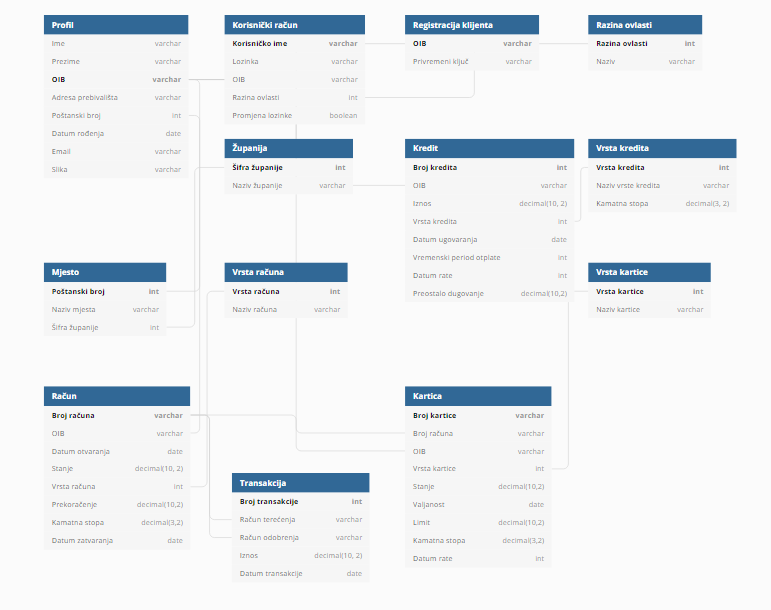
\includegraphics[scale=0.8]{Slike/ermodel.PNG}
					\centering
					\caption{E-R dijagram baze podataka}
					\label{fig:dijagram}
				\end{figure}
			\eject
			
			
		\section{Dijagram razreda}
		
		Na slikama 4.3 - 4.8 prikazani su razredi koji pripadaju backend dijelu MVC
		arhitekture.
		
			\begin{figure}[H]
				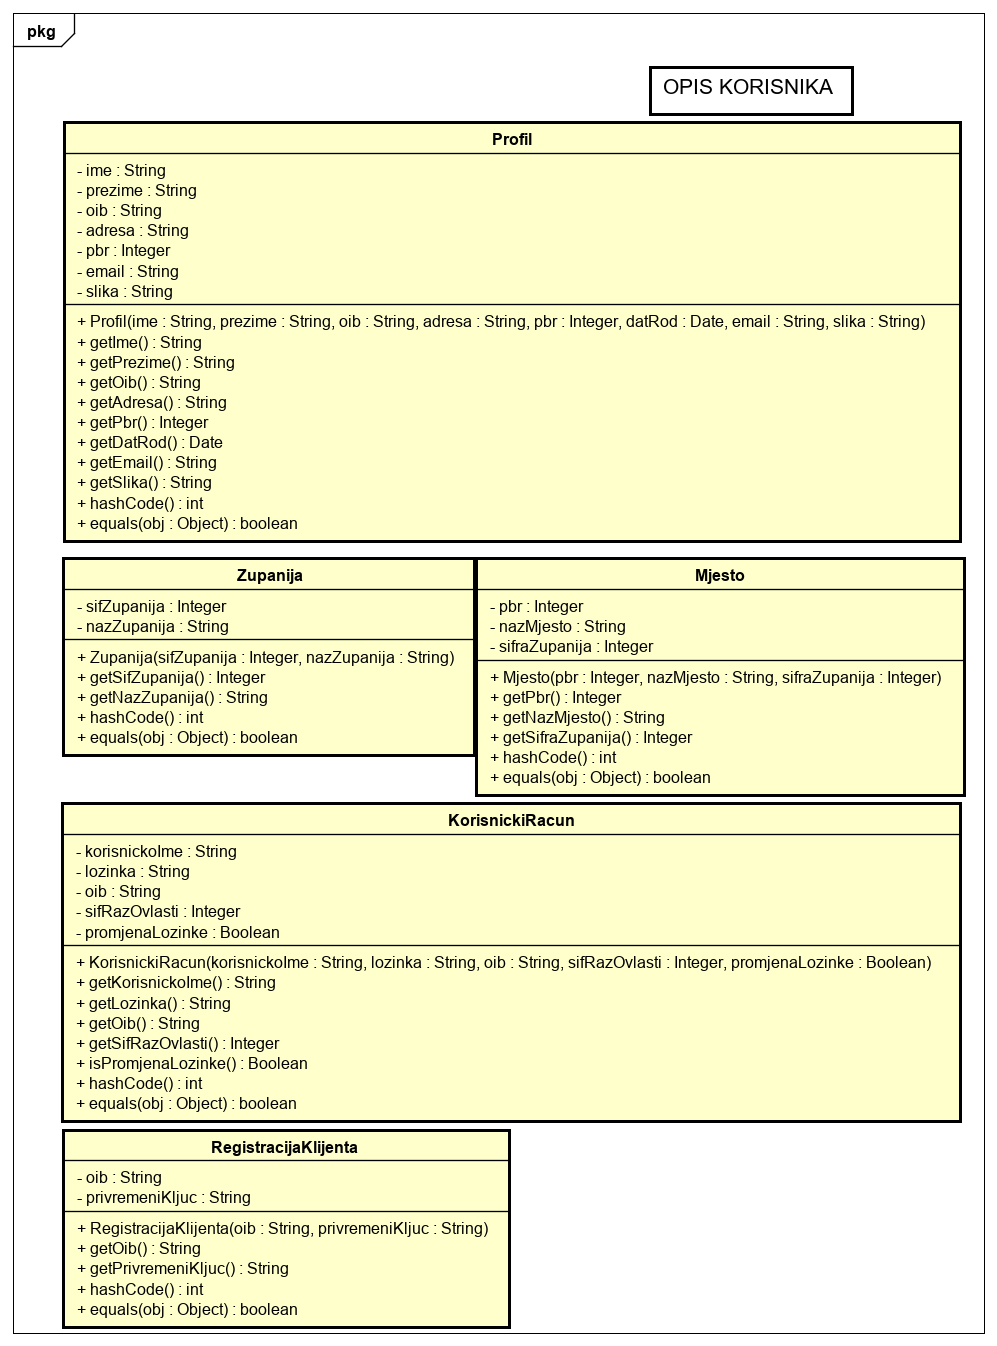
\includegraphics[scale=0.54]{Slike/Class Diagram0.PNG}
				\centering
				\caption{Razredi modela opisa korisnika}
				\label{fig:dijagram}
			\end{figure}
		
			\begin{figure}[H]
				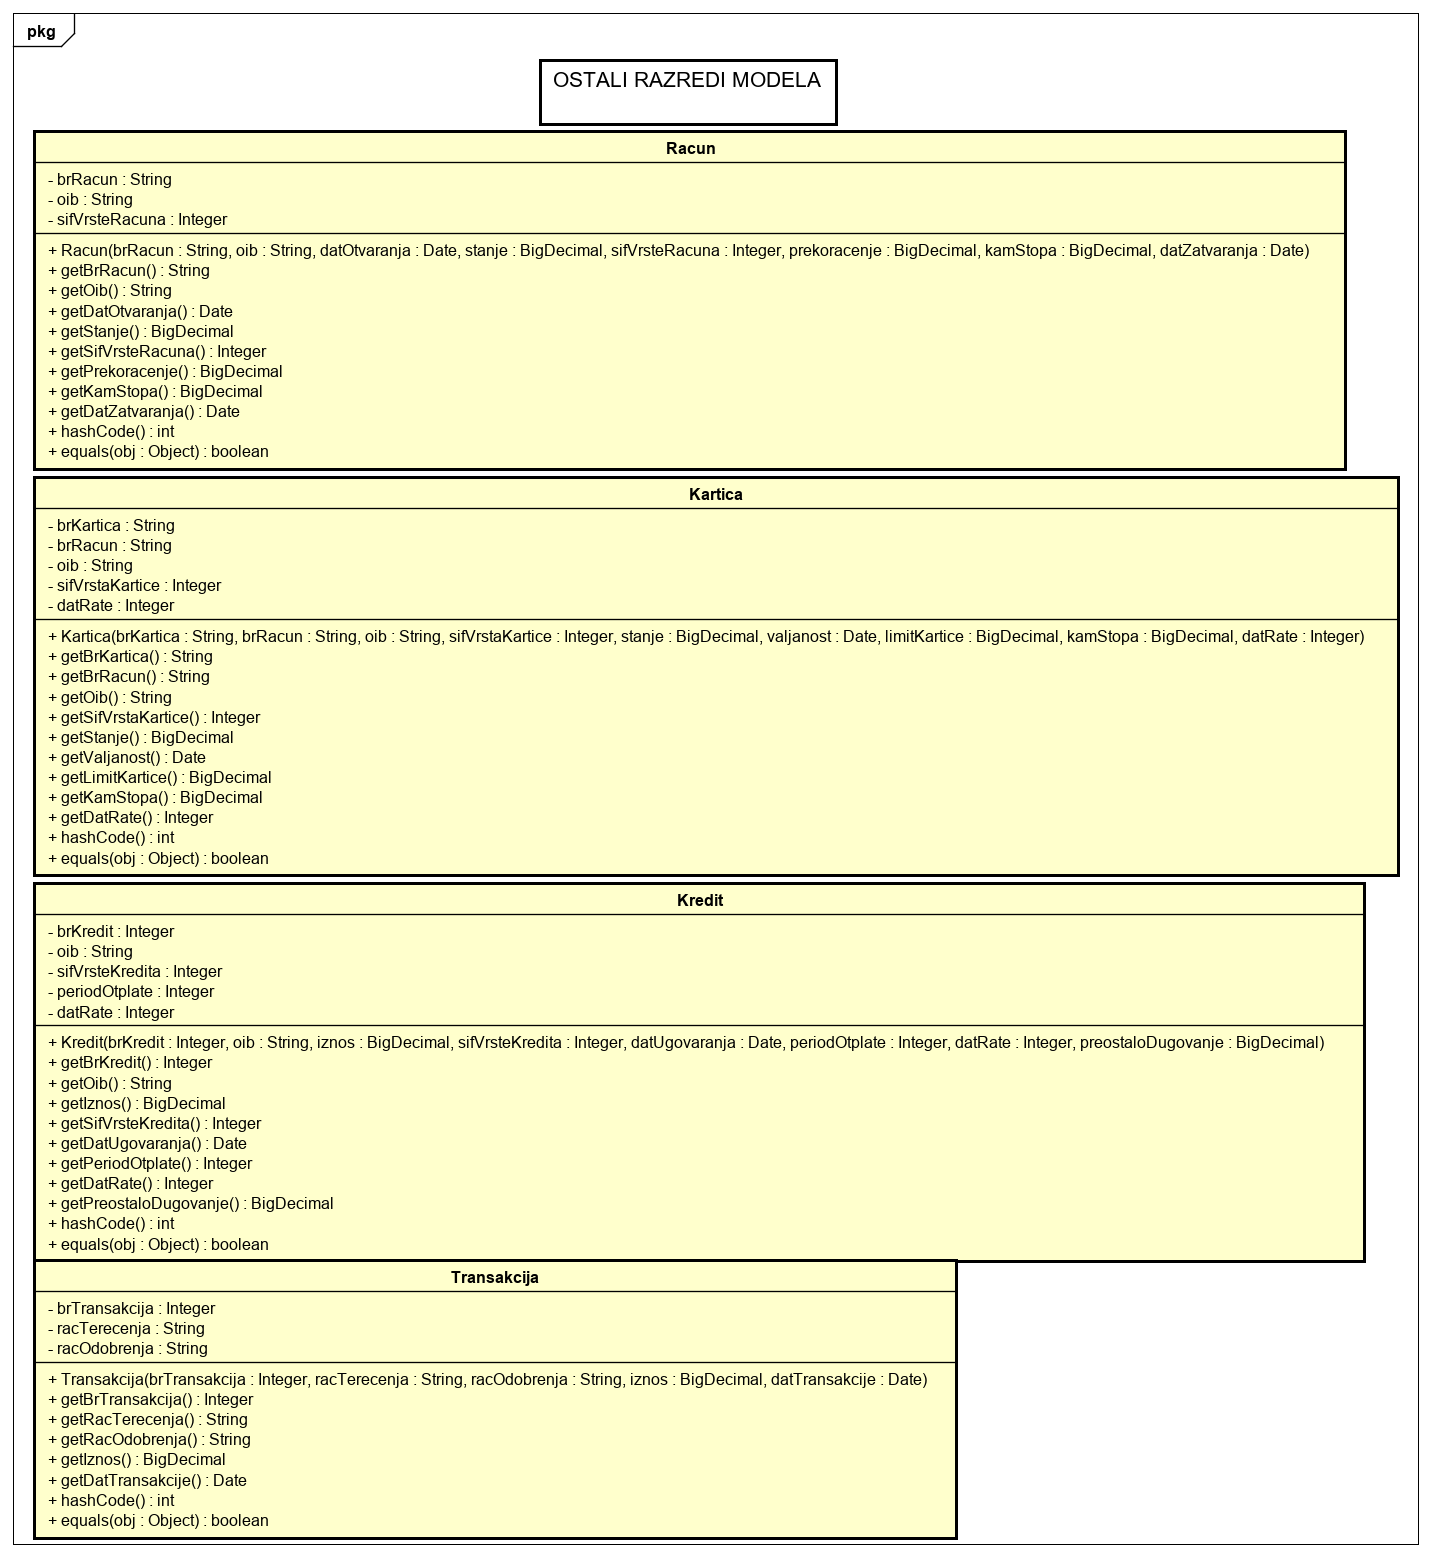
\includegraphics[scale=0.45]{Slike/Class Diagram1.PNG}
				\centering
				\caption{Ostali razredi modela}
				\label{fig:dijagram}
			\end{figure}
		
			\begin{figure}[H]
				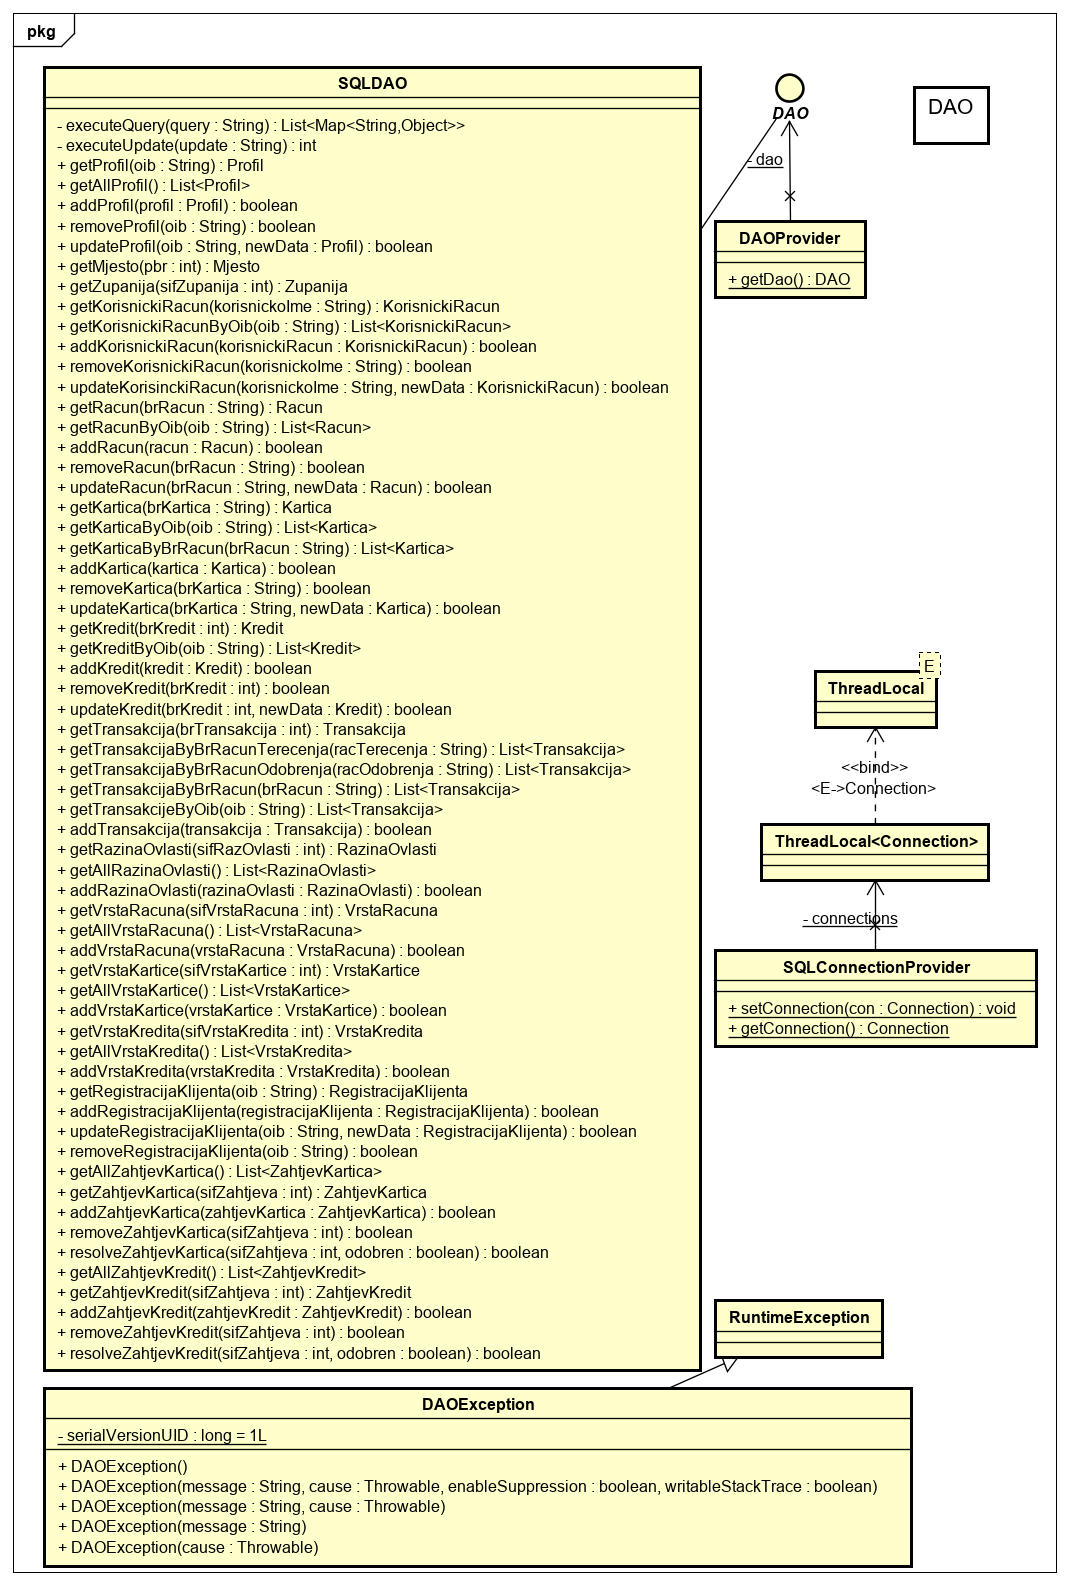
\includegraphics[scale=0.54]{Slike/Class Diagram5.PNG}
				\centering
				\caption{Razredi DAO sučelja}
				\label{fig:dijagram}
			\end{figure}
		
			\begin{figure}[H]
				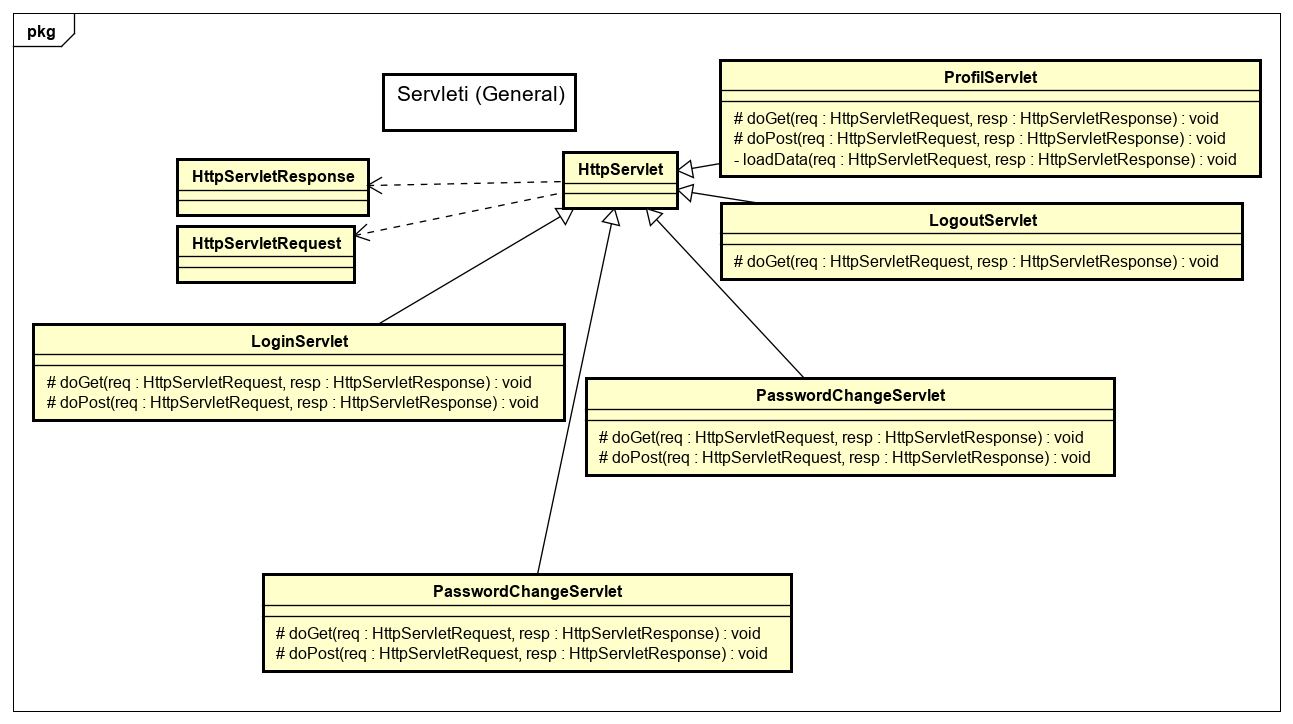
\includegraphics[scale=0.5]{Slike/Class Diagram6.PNG}
				\centering
				\caption{Razredi Servleti prema web sučelju}
				\label{fig:dijagram}
			\end{figure}
		
			\begin{figure}[H]
				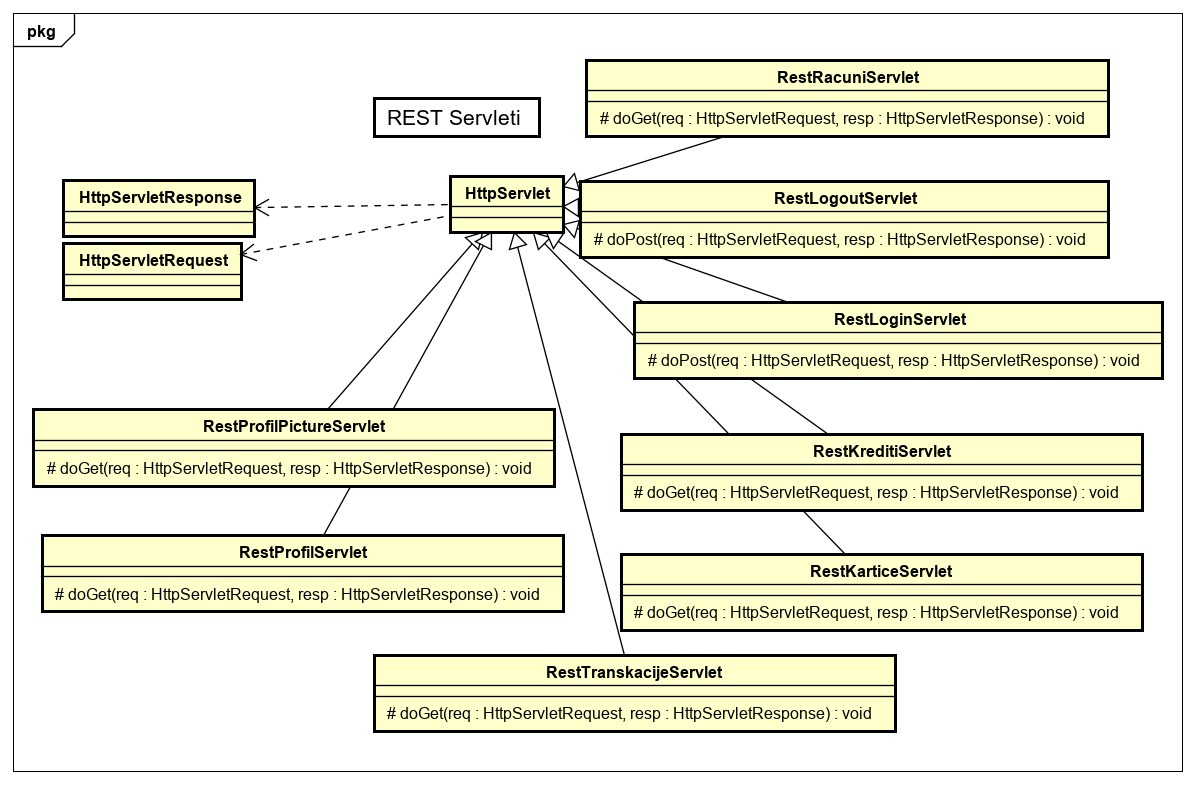
\includegraphics[scale=0.54]{Slike/Class Diagram7.PNG}
				\centering
				\caption{Razredi Servleti RESTful API-a}
				\label{fig:dijagram}
			\end{figure}
		
			\begin{figure}[H]
				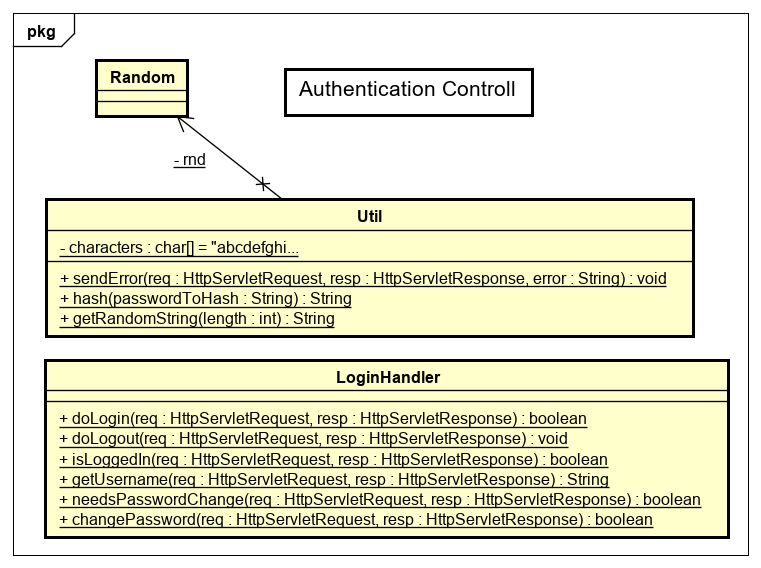
\includegraphics[scale=0.65]{Slike/Class Diagram8.PNG}
				\centering
				\caption{Razredi zaduženi za kontrolu autentifikacije}
				\label{fig:dijagram}
			\end{figure}
		
		\section{Dijagram stanja}
			
			
			
			
			Dijagram stanja spada pod ponašajne i dinamičke dijagrame te prikazuje stanja objekta i prijelaze iz jednog stanja u drugo temeljene na događajima. Na slici 4.9 prikazan je dijagram stanja za registriranog korisnika. Nakon prijave, klijentu se prikazuje početna stranica na kojoj može pregledati svoj profil odnosno osobne podatke. Klikom na "Promijena lozinke" klijent mijenja svoju lozinku. Odabirom "Računa" klijent ima uvid u stanje svojih računa. Klikom na "Kartice" prikazuju mu se podatci o karticama te odabirom "Dodaj karticu" klijent može zatražiti novu kreditnu karticu koju odobrava službenik. Klijent svoje kredite može pregledavati klikom na "Krediti", a odabirom "Novi kredit" poslati zahtjev za novim kreditom službeniku za odobravanje kredita. Klijent odabirom "Otplati kredit" može prijevremeno otplatiti kredit. Pregled transakcija dostupan je klikom na "Transakcije", a klijent može obaviti prijenos sredstava s računa odabirom "Nova transakcija".  
			
			\begin{figure}[H]
				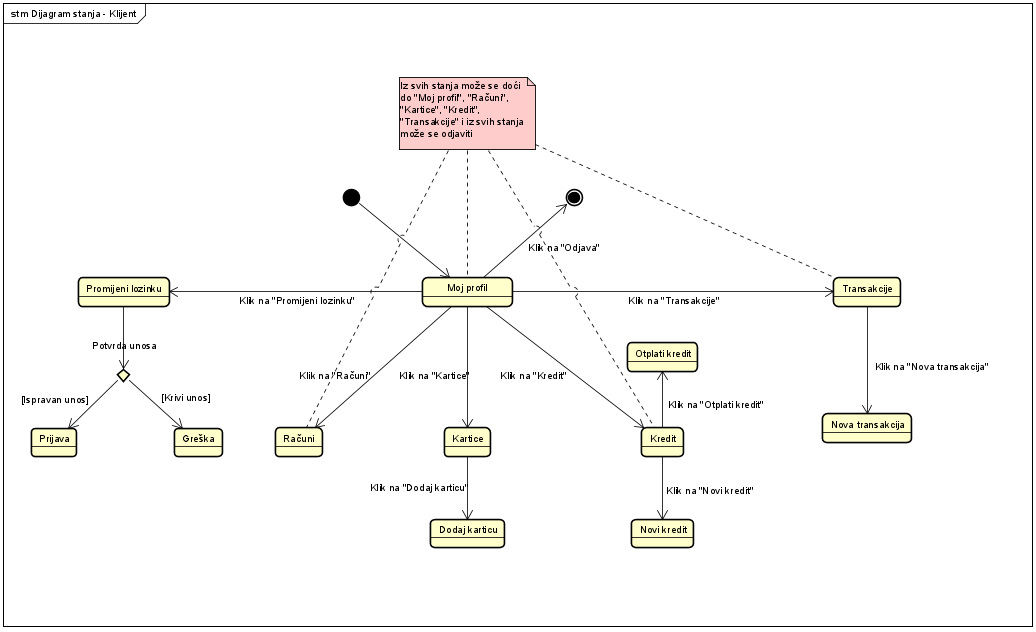
\includegraphics[scale=0.65]{Slike/dijagramStanja.PNG}
				\centering
				\caption{Dijagram stanja}
				\label{fig:dijagram}
			\end{figure}
			
			
			
			
			
		
		\section{Dijagram aktivnosti}
			
			\textbf{\textit{dio 2. revizije}}\\
			
			 \textit{Potrebno je priložiti dijagram aktivnosti s pripadajućim opisom. Dijagram aktivnosti treba prikazivati značajan dio sustava.}
			
			\eject
		\section{Dijagram komponenti}
		
			\textbf{\textit{dio 2. revizije}}\\
		
			 \textit{Potrebno je priložiti dijagram komponenti s pripadajućim opisom. Dijagram komponenti treba prikazivati strukturu cijele aplikacije.}